\documentclass[11pt]{article}
\usepackage[margin=25mm]{geometry}
\usepackage[T1]{fontenc}
\usepackage[utf8]{inputenc}
\usepackage{amsmath,amssymb,graphicx,booktabs,array}
\usepackage{microtype,placeins}
\usepackage[font=small,labelfont=bf]{caption}
\usepackage[colorlinks=true,allcolors=blue]{hyperref}
\newcommand{\gtd}{\ensuremath{\gamma\!\rightarrow\!\delta}}
\newcommand{\dtg}{\ensuremath{\delta\!\rightarrow\!\gamma}}
\title{Additional file 1: supplementary methods and sensitivity analyses}
\author{Zihan He and Jia Meng}
\date{Author-review draft: 9 October 2026}
\renewcommand{\thefigure}{S\arabic{figure}}
\renewcommand{\thetable}{S\arabic{table}}
\begin{document}
\maketitle
\section{Corruption and reconstruction}
Each single-chain sequence is assigned a masking rate of 15\% or 30\% with equal
probability. Exactly the larger of one and the rounded rate times sequence
length is selected without replacement. Each selected residue independently
receives a mask token (80\%), a uniform canonical amino acid (10\%) or its
original token (10\%). Deletion starts are sampled uniformly, with span lengths
uniformly 1--3, until at least the rounded 8\% target is covered; spans can
overshoot that target. Deletion follows masking and can overlap selected sites.
The damaged mask includes selected-but-unchanged residues and deleted sites.
The aligned-copy control copies the corrupted aligned token and uses a mask at
deleted sites. Reconstruction includes EOS in token NLL; residue accuracy is
separately evaluated on original residue positions. No reconstruction metric
is interpreted as partner recovery.

\section{Controls and training}
The conditional and constant-source generators share initialization, target
sampling, optimizer and nominal downstream budget. Constant-source input keeps
the chain token and removes source residues. Random initialization removes
pretraining and retains downstream settings; total training computation is not
matched. Shuffled-input evaluation permutes queries without fixed points and
keeps the original recorded-partner labels. A separate copy of the fine-tuned
generator initializes the ranker. Its copied encoder is trainable; the source
generator is not updated. All paired fits use the same protocol-specific
training edges. Seeds, selected checkpoints and actual exposure accompany
Additional file 3.

AdamW uses weight decay 0.01 and gradient-norm clipping at 1.0. For denoising and
generator training, the per-step learning rate is the nominal rate multiplied
by $\min(1,s/w)$ and $[1+\cos(\pi\min(1,s/S))]/2$, where $s$ is the current
step, $w$ the warmup and $S$ the nominal maximum steps. This applies cosine
decay over the whole nominal run, including warmup. Ranker training uses its
fixed stated learning rate. Training may stop early; actual exposures, not only
nominal limits, are retained.


\begin{table}[htbp]
\centering
\caption{Core generator controls. All conditions retain the protocol-specific test query population and fixed primary sampling rule.}
\begin{tabular}{p{0.30\linewidth}p{0.64\linewidth}}
\toprule
Condition & Comparison purpose\\
\midrule
Pretrained conditional & Uses the input chain after denoising pretraining.\\
Constant-source target prior & Removes source residues while matching initialization, target sampling and downstream optimization.\\
Random initialization & Removes denoising pretraining; the downstream budget is matched, total computation is not.\\
Shuffled input & Breaks the input--recorded-partner association at evaluation using the fitted conditional model.\\
\bottomrule
\end{tabular}
\end{table}

\section{Constructed negatives and candidate construction}
The primary ranker first uses multi-positive contrastive training, then equally
weighted positive and constructed-negative binary cross-entropy. Three negative
draws per positive are drawn from supervised-training combinations, excluding
known training partners. The mixed policy combines random and length/terminal
matching; actual fallbacks and draw counts are recorded. Unrecorded combinations
are not biological negatives. Sensitivities change ratios to one or five, or
use random-only draws. Fixed retrieval pools inject all role-specific recorded
positives and up to 100 unrecorded targets from that role's universe. Other
recorded partners are excluded from distractors. Random, length, terminal-motif
and normalized-edit matching are deterministic at fixed seed. All scorers use
the same frozen lists. Free sampling instead makes 64 draws with temperature
one and top-p 0.95; 6--35 canonical residues and observed EOS are required.
Invalid and duplicate draws are never replaced. Training-target exclusion is
an explicitly separate policy that can delete legitimate exposed positives.

For each negative draw, the source direction is chosen with equal probability.
Under the mixed policy, a hard draw is chosen with probability 0.5. Candidate
training targets within one residue of the reference target length are sorted
by absolute length difference, mismatch count over the first and last three
residues, then sequence. The draw is uniform over the first 64 eligible targets
after known-training-partner exclusion. If none remain, sampling falls back to
uniform random eligible training targets. Sampling is with replacement;
no held-out pairing labels filter training negatives. The two BCE classes each
receive one-half of the loss weight at every negative ratio.

Fixed-pool length matching sorts eligible role targets by the minimum length
gap to a role-specific positive, then normalized full-CDR3 edit distance and
sequence. Motif matching uses the sum of Levenshtein distances over the first
and last three residues, then full normalized edit distance and sequence. Edit
matching uses full normalized distance and sequence. Random pools sample
without replacement. Candidate targets are lexicographically stored, and score
ties use that order. Truth-containing retrieval is an explicitly constructed
diagnostic; no such positive-directed pool construction is used in free sampling.

\section{Uncertainty and event reporting}
Query-macro metrics weight inputs equally, with directions averaged equally for
the primary endpoint. The bootstrap uses 2000 resamples of complete test graph
components, shared across directions and paired model contrasts. Directional
tasks use source-query groups. The repair of unseen-gamma selection retains
this directional uncertainty unit. The within-giant-component experiment has
one original component and reports no inferential interval. Intervals condition
on fitted models and saved samples, without multiplicity adjustment. A zero-event
[0,0] interval is not a population upper bound. Across primary splits, seeds
are averaged first and the three split means have a descriptive SD; neither
fits nor repeated splits are independent biological replicates.

\section{Pretraining and negative-sampling sensitivity}
\subsection{Pretraining mixture and downstream sampling have distinct effects}
The two-seed downstream NLL means for square-root, raw and balanced pretraining
are, respectively, 1.256/0.754, 1.255/0.757 and 1.259/0.755 for \gtd{}/\dtg{}
on split 17 (Figure~\ref{fig:figure_S1_pretraining}). Raw-minus-square-root
equal-direction differences are approximately 0.001 nats per token in both
fits, with paired intervals crossing zero. Balanced-minus-square-root
differences are approximately 0.002 in both fits, with intervals above zero.
These small NLL differences do not select a new primary mixture after testing.

Restricting pretraining to one chain has larger directional effects. Gamma-only
initialization gives downstream NLL 1.294/0.755, while delta-only initialization
gives 1.257/0.779. On frozen denoising validation, gamma-only pretraining yields
39.6\% selected-site accuracy for delta, and delta-only pretraining yields
27.3\% for gamma, compared with 64.4\% and 70.8\% under the square-root
mixture. The results are consistent with chain-specific reconstruction exposure
affecting the target-sequence prior. Equal total sequence draws do not equate
chain-specific or token exposure, and these teacher-forced differences do not
demonstrate reliable free partner recovery.

Edge-uniform paired training gives NLL 1.263/0.759, compared with 1.256/0.754
under query-uniform training. Its equal-direction excess is approximately
0.006 nats per token in both fitted seeds, with paired intervals above zero.
The nominally direction-budget-matched unidirectional models give NLL
1.258 for \gtd{} and 0.756 for \dtg{}, close to the bidirectional model.
All these settings retain sparse free-recovery events. Their actual early-stop
and token exposure records accompany the matched nominal budgets; the comparison
does not establish a universal benefit from sharing the two directions.

\begin{figure}[!htbp]
\centering
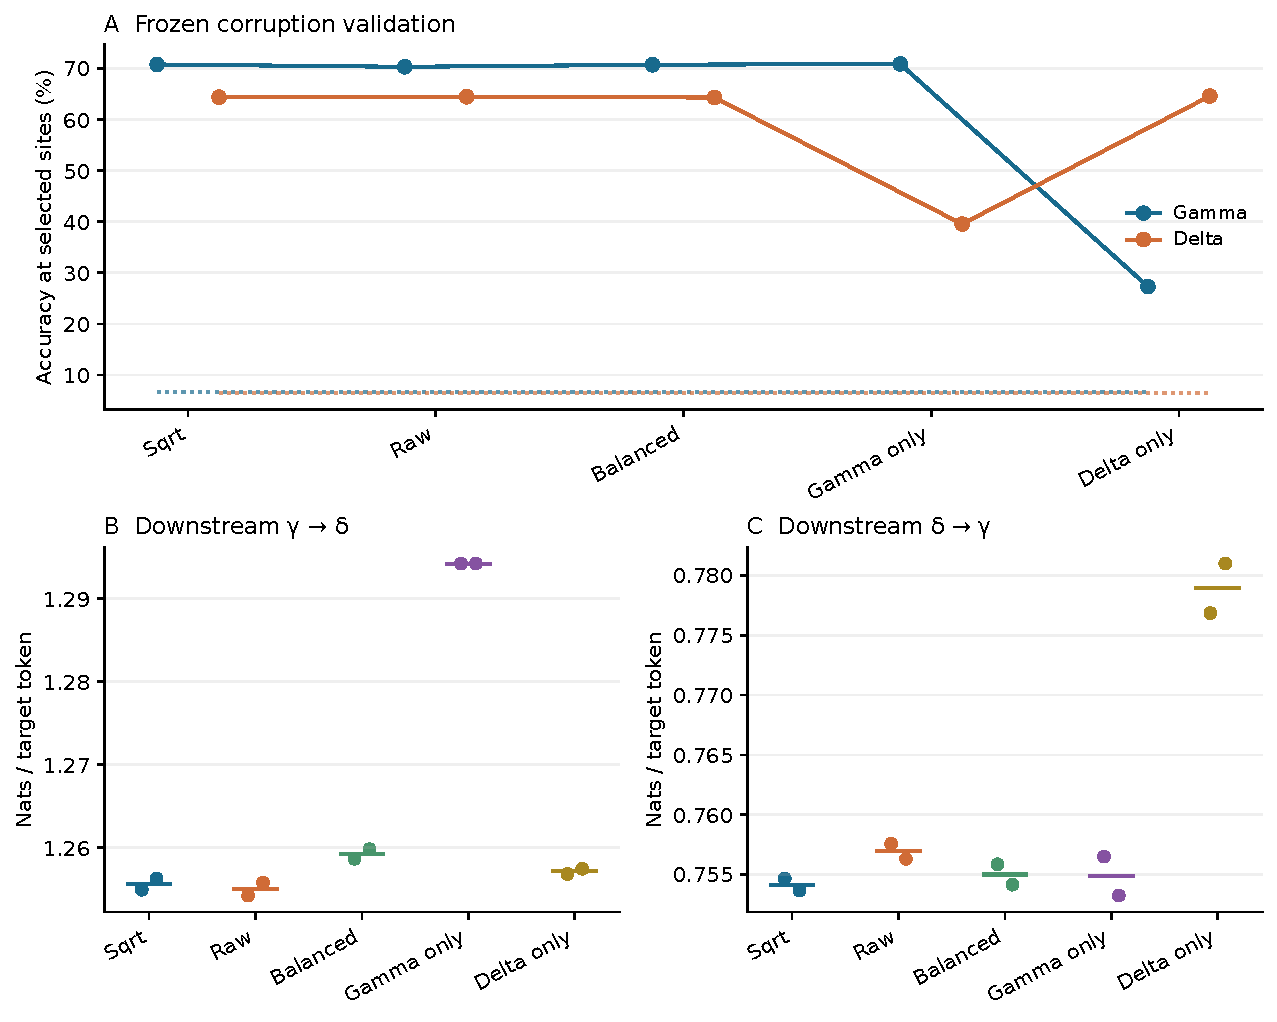
\includegraphics[width=\linewidth]{results/bmc/figures/figure_S1_pretraining.pdf}
\caption{Pretraining mixture sensitivity. Dots retain fitted seeds. Equal sequence draws do not imply equal chain-specific or token exposure. Reconstruction is a single-chain endpoint.}
\label{fig:figure_S1_pretraining}
\end{figure}
\FloatBarrier

\subsection{Changing negative training does not resolve candidate scarcity}
Random-only and mixed negative training at ratios one, three and five reuse the
same split-17 generator candidates and retrieval pools
(Figure~\ref{fig:figure_S2_negative_training}). All twelve fitted rankers have
zero free-generation \gtd{} Hit@5. For \dtg{}, individual fitted values range
from zero to 0.22\% (zero to two of 900 queries), with no monotonic gain from
increasing the ratio. The primary mixed/3 setting averages 0.11\%; random/5,
mixed/1 and mixed/5 each average 0.17\%. Such small event differences do not
establish a reproducible recovery advantage: paired intervals for every
alternative negative setting versus the primary setting include zero in both
directions and both fitted seeds.

Fixed-pool differences are larger but depend on the comparison. In random
retrieval pools, random/3 gives two-seed mean ranker Hit@5 of 10.8\% for
\gtd{}, compared with 8.2\% under mixed/3. For \dtg{}, random/5 gives
9.1\%, compared with 7.1\% under mixed/3. These descriptive rankings are not
uniform across pools or seeds, and no setting supplies candidates absent from
the frozen free-generation set. Negative-draw and fallback counts, selected
steps and paired contrasts are retained in the numerical supplement. None of
these constructed-negative comparisons identifies biological incompatibility.


\begin{figure}[!htbp]
\centering
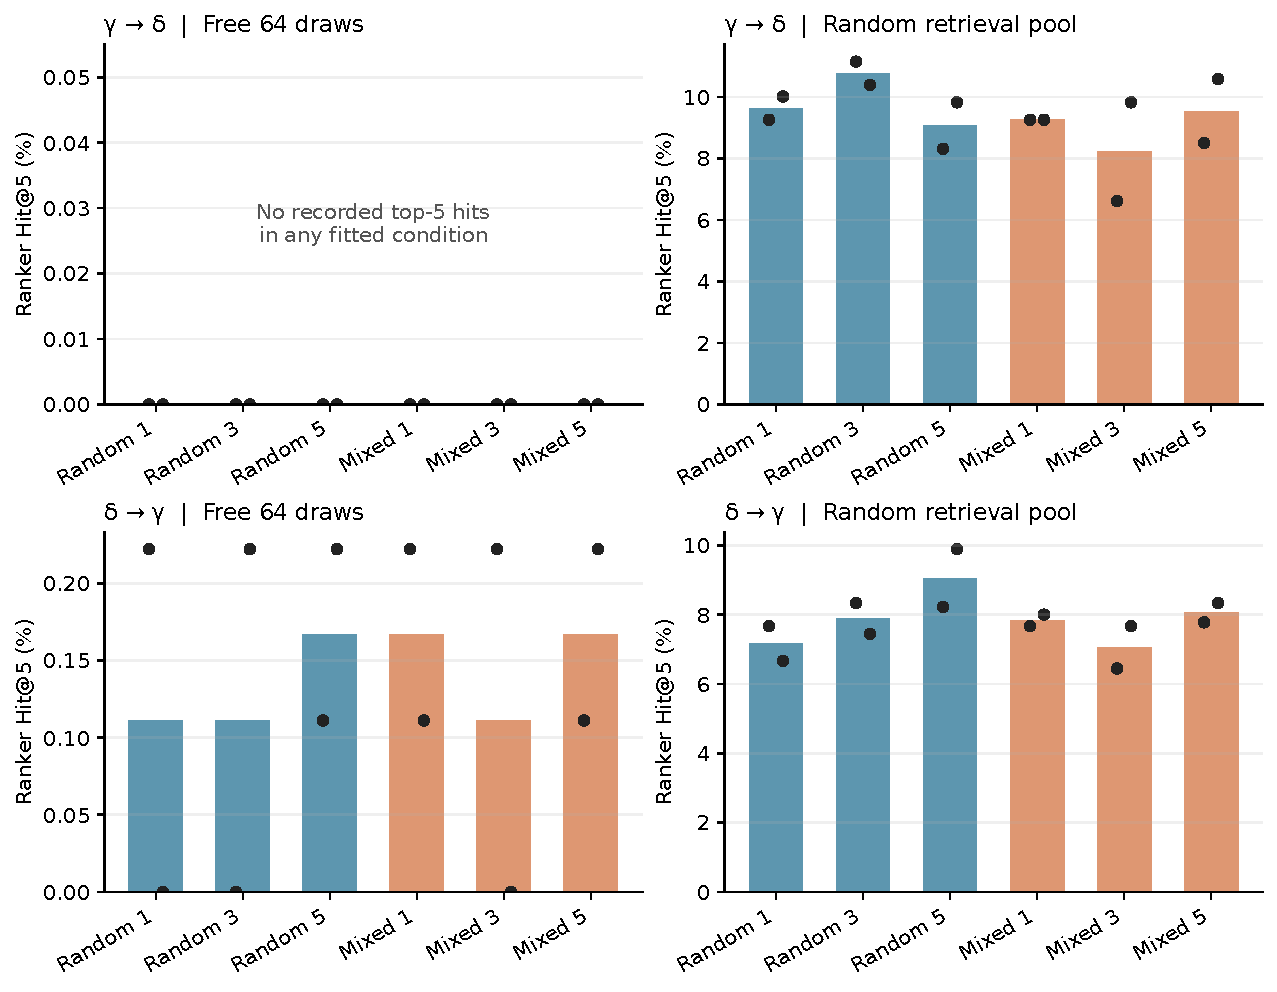
\includegraphics[width=\linewidth]{results/bmc/figures/figure_S2_negative_training.pdf}
\caption{Ranker negative-sampling sensitivity. All settings reuse the same saved free candidates and frozen truth-containing retrieval pools. No ranker adds absent candidate sequences.}
\label{fig:figure_S2_negative_training}
\end{figure}
\FloatBarrier

\section{Nearest-input baselines and exposure diagnostics}
Nearest-input transfer uses the normalized full-CDR3 distance, lexicographic
input ties and training-degree/lexicographic target ordering. One nearest
input is primary; five is a fixed sensitivity. At most 64 unique training
targets are returned. In seen-input/withheld-edge tasks the exact input is its
own nearest neighbor, so one-neighbor transfer cannot recover its withheld
edges. Primary component-disjoint transfer is also structurally zero because
all test targets are absent from training. These zero outcomes do not identify
a learned-model mechanism. The separate nearest-input partner-similarity retrieval
score extends to the role-specific target universe using minimum target edit
distance to the nearest input's known training partners. Neither neighborhood
size nor distance rule was selected using test outcomes. Test memberships,
selection repairs and the giant-component edge reservation are frozen in the
revision split manifest. These are post-primary revision diagnostics.

\subsection{Unseen-gamma validation design and historical estimates}
The original selection partition contained one gamma query with 581 recorded
partners and no ranking distractors. Its ranker selection MRR was identically
one. Original conditional likelihood Hit@5 was 9/64 in each seed (14.06\%),
compared with 9/64 and 8/64 for constant source (14.06\%/12.50\%). These
estimates are retained for traceability, not as robust unseen-gamma evidence.
The repaired-selection refits preserve the original train, aggregate validation
and test memberships and replace this diagnostic in the main text. Primary
component-disjoint results remain unchanged. The revised selection has 31
gamma queries, 275 edges, a largest query with 137 partners and at least 118
eligible distractors per query. The tuning and calibration roles each contain
16 disjoint gamma queries and are not used for new tuning in this revision.

\subsection{Source and component-stratified descriptive analyses}
Additional file 2 includes primary source and source-distance strata and a
post-hoc source-balanced description. The latter averages nonempty source
membership strata equally. Memberships can overlap, and very small source
strata are unstable; this is neither a reweighted primary endpoint nor a
source-independent inferential comparison. Post-hoc component-size tables group
primary-test components into 1, 2--5, 6--20 and more than 20 edges, retaining
the original query positives and saved candidates. Nonempty bins give counts
and descriptive means without inferential intervals. The distant-edge recheck recovers
5, 5 and 3 primary edges, with no new claim of distant-sequence transfer.
Within-giant-component estimates originate from one original component and
deliberately have no inferential interval. Additional file 4 retains every
revision query outcome, including zero events, all control conditions and
paired contrasts. Additional file 3 records actual generator sequences and
target tokens; ranker encoded-token counts were not logged and are not imputed.


\end{document}
